\documentclass[a4paper]{scrreprt}

\usepackage{listings}
\usepackage{color}
\usepackage{textcomp}
\usepackage{hyperref}
\usepackage[english]{babel}
\usepackage{graphicx}
\usepackage{float}
\usepackage{caption}
\usepackage{subcaption}
\usepackage[section]{placeins}
\usepackage{multirow}

\definecolor{listinggray}{gray}{0.9}
\definecolor{lbcolor}{rgb}{0.9,0.9,0.9}
\lstset{
	language=C++,
	keywordstyle=\bfseries\ttfamily\color[rgb]{0,0,1},
	identifierstyle=\ttfamily,
	commentstyle=\color[rgb]{0.133,0.545,0.133},
	stringstyle=\ttfamily\color[rgb]{0.627,0.126,0.941},
	showstringspaces=false,
	basicstyle=\small,
	numberstyle=\footnotesize,
	numbers=left,
	stepnumber=1,
	numbersep=10pt,
	tabsize=2,
	breaklines=true,
	prebreak = \raisebox{0ex}[0ex][0ex]{\ensuremath{\hookleftarrow}},
	breakatwhitespace=false,
	aboveskip={1.5\baselineskip},
  columns=fixed,
  upquote=true,
  extendedchars=true,
% frame=single,
% backgroundcolor=\color{lbcolor},
}    

\title{CGoGN plug}
\author{Hurstel Alexandre}
\subtitle{A quick SOCIC2012 project overview\\+\\how to use}
\begin{document}

\maketitle

\tableofcontents

\chapter{Introduction and purposes}

\section{CGoGN}
\subsection{What is CGoGN library ?}
	\paragraph{}
	\textbf{CGoGN} is a C++ topological geometric modeling kernel that provides
	efficient and generic data structures based on n-dimensional combinatorial maps.

	\paragraph{}
	The main purpose of \textbf{CGoGN} is to provide a strong separation between
	the description of the topology of the mesh (the cells and their adjacency
	relationships) and the space in which the cells are embedded (attributes
	associated to the cells) in the meantime the library also provides efficiency
	(more contiguous tables, less pointers), low memory consumption, genericity
	(models, dimensions).
	
	\paragraph{}
	A good start to get familiar with \textbf{CGoGN} and all of its features is to
	get familiar with \href{http://en.wikipedia.org/wiki/Topology}{topology} and
	check the \href{http://cgogn.u-strasbg.fr/Wiki/index.php/CGoGN}{\textbf{CGoGN}
	project page}.
	
\subsection{CGoGN and visualization?}
	\paragraph{}
	Since \textbf{CGoGN} is a topological library, it has to provide graphical
	tools to visualize the topological models it allows to generate although it's
	not quite its priority concern.
	
	\paragraph{}
	That's why the \textbf{CGoGN} library provides some useful tools of
	visualization that take forms of C++ classes that are actually inheritance or
	implementation of \href{http://qt-project.org/}{\textbf{Qt} framework}'s C++
	classes. Within the same state of mind, the library also provides easy to use
	C++ rendering functions and classes that operate several
	\href{http://www.opengl.org/}{\textbf{OpenGL}} features and functions.
	
\section{The project}
\subsection{CGoGN in space?}
	\paragraph{}
	The aim of this project is not to replace or improve any of the \textbf{CGoGN}
	rendering classes of functions, but to use these provided features to create
	and implement a new approach to provide visualization for \textbf{CGoGN}'s
	objects.
		
	\paragraph{}
	With the current GUI tools provided by \textbf{CGoGN}, the programmer using the
	library generally has to inherit some classes that are themselves inheritance of
	some \textbf{Qt} GUI classes (see the
	\href{http://cgogn.u-strasbg.fr/Wiki/index.php/Doc_qt}{SimpleQt example}).
	Doing so, he will create a new and independent application.
	The main idea of the project is to allow the coder, not to create his own
	application, but to write code and add it dynamically to a main application,
	already containing basics GUI features.
	
\subsection{Plugins and CGoGN?}
	\paragraph{}
	In order to offer such a system, the goal of the project was to provide CGoGN
	with an application that integrates a \textbf{plugin system}. This means that
	any coder could develop is own third party code as a compatible plugin and add
	it to the main application as a new feature, without ever touching the main
	application's inner code or even without having to recompile it.
	
	\paragraph{}
	The function of the main application is to provide visualization (with several
	functionalities) of CGoGN generated objects combined with a few possibilities
	of GUI to interact with these. However, the application itself, without any plugin attached to it,
	doesn't give any visualization or relevant interface. Although the application
	provide this functionalities, they have to be activated and called by the
	plugins that will be attached to the application. As a metaphor, the main
	application is like an empty house with electricity and running water, but that
	has to be filled with various furniture, appliance, decoration, etc\ldots
	
	
	
\chapter{The project}

\section{Work}
\subsection{Specifications}
	\paragraph{}
	The project was developed to meet several specifications:	
	\begin{itemize}
	  \item The plugins can provide a drawing function for the application to show
	  \item Several cameras can show at the same time a 3D visualization from a
	  different point of view.
	  \item The application can show several different visualization at the same
	  time.
	  \item A plugin draw function can complete another plugin's draw function.
	  \item The plugins can add entries in the application menus
	  \item The plugins can add their own widgets in a dedicated area of the
	  application (typically a dock).
	  \item A plugin can provide a map
	  (\href{http://en.wikipedia.org/wiki/Topological_map}{see topological maps}
	  and
	  \href{http://cgogn.u-strasbg.fr/Wiki/index.php/Topological_models}{CGoGN's
	  map}) that could be shared/reused by other plugins.
	\end{itemize}
	
\subsection{Additional features}
	\paragraph{}
	In addition to the previous specifications it was also appreciate that the
	project could be completed with some features that are:
	\begin{itemize}
	  \item A path for the cameras in a 3D scene could be interpolated from
	  successive camera positions so that the camera could follow that path while
	  she saves snapshots during its movement.
	  \item A map could be imported from external files.
	\end{itemize}
	Those additional features, were developed as plugins for the application
	since they are not primary needed features.

\subsection{Third party libraries}
	\paragraph{}
	In order to implement the required features of the project in an easy and
	effective way, the project naturally uses third party libraries. Without
	considering the many third party libraries already used in \textbf{CGoGN}, the
	work was done using mainly two libraries:
	\begin{itemize}
	  \item \textbf{\href{http://qt-project.org/}{Qt}}: the effective and popular
	  framework, which, thus providing all the GUI features, provides the kernel
	  for our project's plugin system using
	  \href{http://qt-project.org/doc/qt-4.8/plugins-howto.html#the-lower-level-api-extending-qt-applications}{Qt's
	  plugin framework}.
	  \item \textbf{\href{http://www.libqglviewer.com/}{libQGLviewer}}: A library
	  that is also based on Qt, but that provides interesting efficient visualization
	  features especially regarding camera gesture.
	\end{itemize}
	
\section{Quick presentation}
	\paragraph{}
	This section quickly presents the main application interface then the use of
	the	\textit{importMap} and the \textit{cameraPath} plugin.
	
\subsection{The main application}
	\paragraph{}
	\begin{figure}[h!p]
	Here's the main application after a first launch.
	  \centering
	    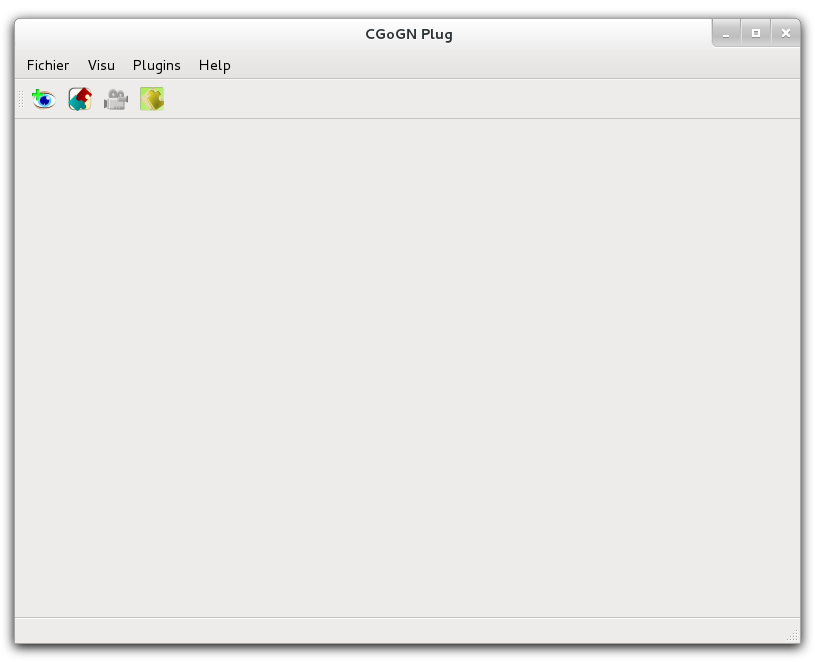
\includegraphics[width=0.7\textwidth]{images/screenshot1}
	  \caption{The main window application without any plugin loaded or used.}
	\end{figure}
	\begin{figure}[h!p]
	Now we need to load a plugin.\\
	  \centering
	    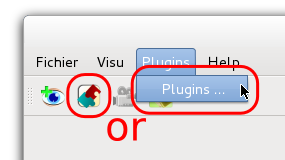
\includegraphics[width=0.5\textwidth]{images/screenshot2}
	  \caption{Load the plugin button.}
	\end{figure}
	\begin{figure}[h!p]
	We then choose a plugin to load. Plugins are particular C++ dynamic libraries,
	they take the form of \textit{lib*.so} files. For example, here we want to load
	a plugin called \textit{tuto5Geom} so we select he file \textit{libTuto5Geom.so}.
	Custom plugin directories or, individual plugin files can be specified from
	this interface.\\
	  \centering
	    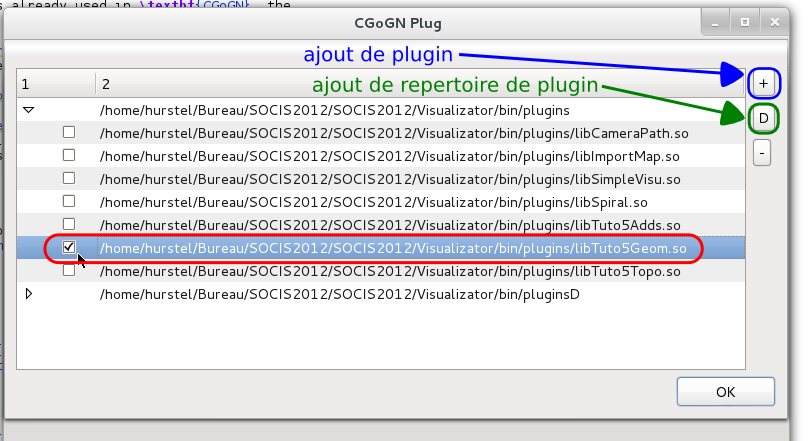
\includegraphics[width=0.95\textwidth]{images/screenshot3}
	  \caption{Load plugins interface.}
	\end{figure}
	\begin{figure}[h!p]
	Our plugin is loaded, but nothing happened. This plugin is a visualization
	plugin: it provides a visualization of a grid cube. We don't have yet any
	visualization because, most plugins generally wait to be associated with a
	scene to draw in, so we still have to create a scene manually. (Note that
	plugins could create their own scene automatically, if the plugin creator
	wants to, but this approach is discouraged)\\
	  \centering
	    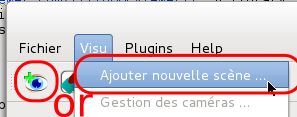
\includegraphics[width=0.6\textwidth]{images/screenshot4}
	  \caption{Adding scenes button.}
	\end{figure}
	\begin{figure}[h!p]
	We now chose a name for our view, and chose to link it with an existing
	previously load plugin. Note that a view can be linked to a plugin even after
	its creation.\\
	  \centering
	    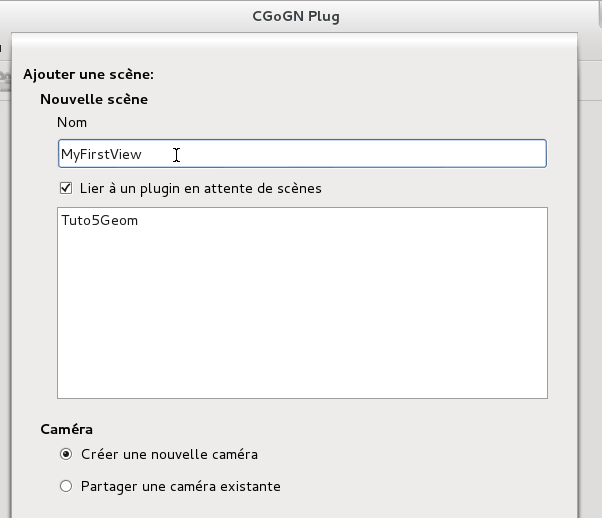
\includegraphics[width=0.95\textwidth]{images/screenshot5}
	  \caption{Adding scenes interface.}
	\end{figure}
	\begin{figure}[h!p]
	And here's the view with our drawing.\\
	  \centering
	    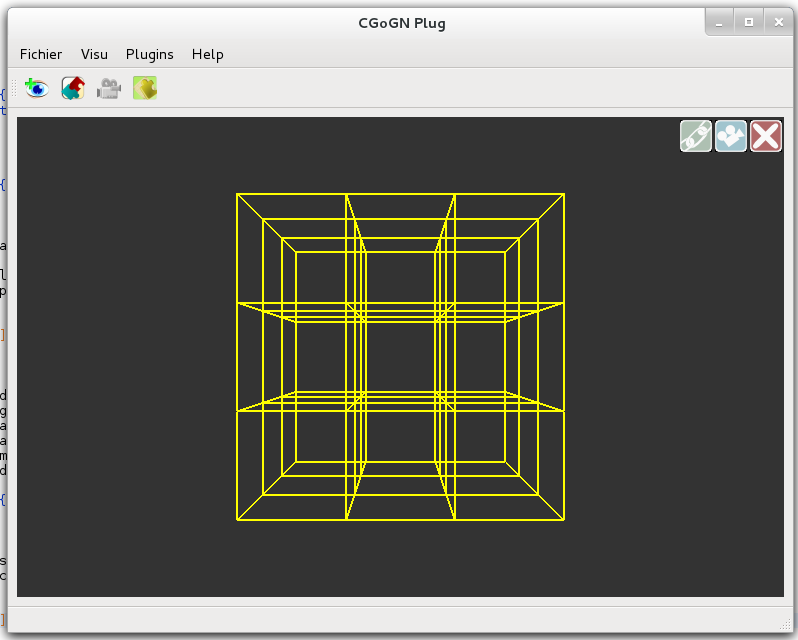
\includegraphics[width=1\textwidth]{images/screenshot6}
	  \caption{A scene associated to a drawing plugin.}
	  \label{fig:tuto5GeomView}
	\end{figure}
	\begin{figure}[h!p]
	Let's now watch this scene from two different points of view. Several step have
	to be made: first we have to create a new camera.\\
	  \centering
	    
\includegraphics[width=0.3\textwidth]{images/screenshot7}
	  \caption{View's camera gesture for this scene.}
	\end{figure}
	\begin{figure}[h!p]
	  \centering
	    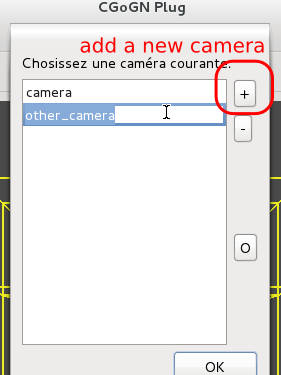
\includegraphics[width=0.5\textwidth]{images/screenshot8}
	  \caption{Creating and naming a new camera.}
	\end{figure}
	\begin{figure}[h!p]
		We now have a single view with two cameras. We're going to separate these two
		cameras into two different views, and by doing so splitting this scene into
		two views.\\
	  \centering
	    
\includegraphics[width=0.3\textwidth]{images/screenshot9}
	  \caption{View management button.}
	\end{figure}
	\begin{figure}[!]
	We create a new view for this scene, then we drag'n drop one of the two cameras
	into this new view.\\
        \begin{subfigure}[h!p]{0.6\textwidth}
                \centering
       		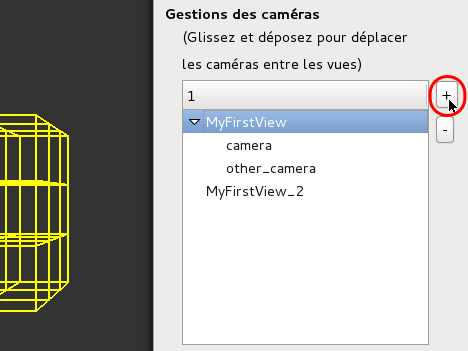
\includegraphics[width=\textwidth]{images/screenshot10}
        \end{subfigure}
        ~
        \begin{subfigure}[h!p]{0.5\textwidth}
                \centering
        	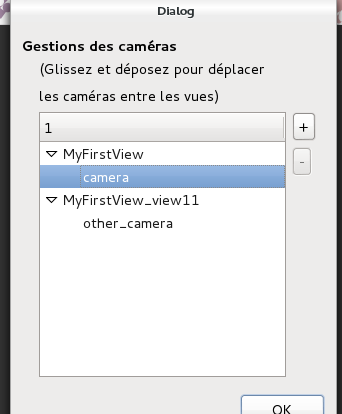
\includegraphics[width=\textwidth]{images/screenshot11}        
        \end{subfigure}
	\end{figure}
	\begin{figure}[h!p]
	We now have the same scene that can be viewed by two different points of
	view.\\
	  \centering
	    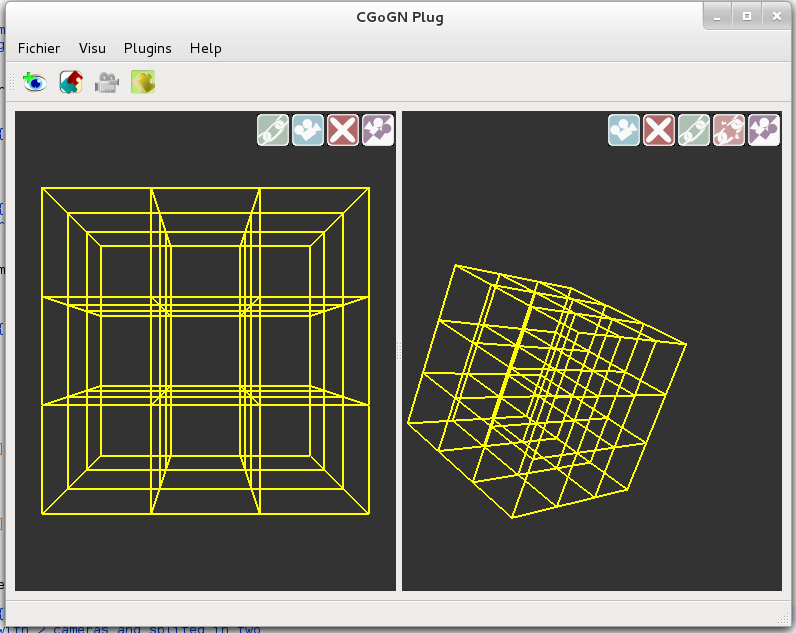
\includegraphics[width=0.95\textwidth]{images/screenshot12}
	  \caption{1 plugin drawing in one scene with 2 cameras and split into 2
	  view.}
	  \label{fig:tuto5GeomDoubleView}
	\end{figure}
	
	\FloatBarrier
\subsection{The import plugin}
	\paragraph{}
	The import plugin is a plugin that loads a map form a \textit{.off} file, and
	then references it within the main application so that it can be given to other
	plugins and reused by them.
	\begin{figure}[h!p]
		Loading the \textit{importMap} plugin.
	  \centering
	    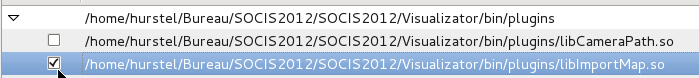
\includegraphics[width=0.9\textwidth]{images/screenshot13}
	  \caption{Loading the «importMap» plugin.}		
	\end{figure}
	\begin{figure}[h!p]
		This plugin doesn't provide any visualization function, it just loads map into
		memory, that's why we don't (and can't) link it to any view. Once loaded the
		plugin adds an ``\textit{import map}'' option to the menu and/or toolbar.\\
	  \centering
	    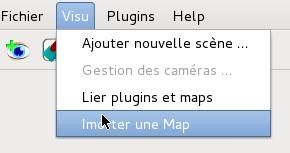
\includegraphics[width=0.4\textwidth]{images/screenshot14}
	  \caption{A wild menu entry appears!}	
	\end{figure}
	\begin{figure}[h!p]
		We now chose an \textit{.off} file to load.\\
		\centering
	    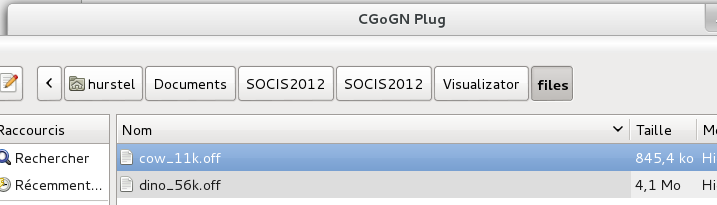
\includegraphics[width=0.9\textwidth]{images/screenshot15}
	  \caption{File dialog.}			
	\end{figure}
	\begin{figure}[h!p]
		The map is now loaded in memory, but we need a tool to visualize it. Skipping
		the procedure that is the same as before, we load the ``\textit{simpleVisu}''
		plugin, and link a new scene to it. But we still have to tell the
		``\textit{simpleVisu}'' plugin, to use this map.\\
		\centering
		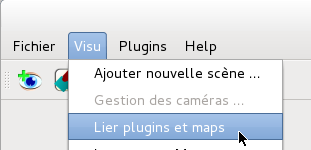
\includegraphics[width=0.6\textwidth]{images/screenshot16}
		\caption{Link map and plugin menu entry}
		\label{fig:linkMapPlugin}
	\end{figure}
	\begin{figure}[h!p]
		We select the concerned plugin, then we double click on the available maps
		list. The green icon indicates that the map is linked with the selected
		plugin.\\
		\centering
		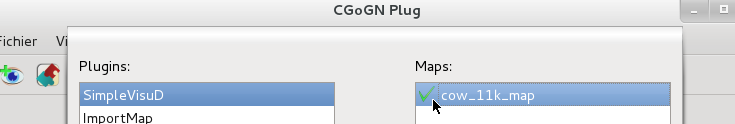
\includegraphics[width=0.95\textwidth]{images/screenshot17}
		\caption{Link map and plugin menu entry}
	\end{figure}
	\begin{figure}[h!p]
		And we have a visualization of our loaded map.
		\centering
		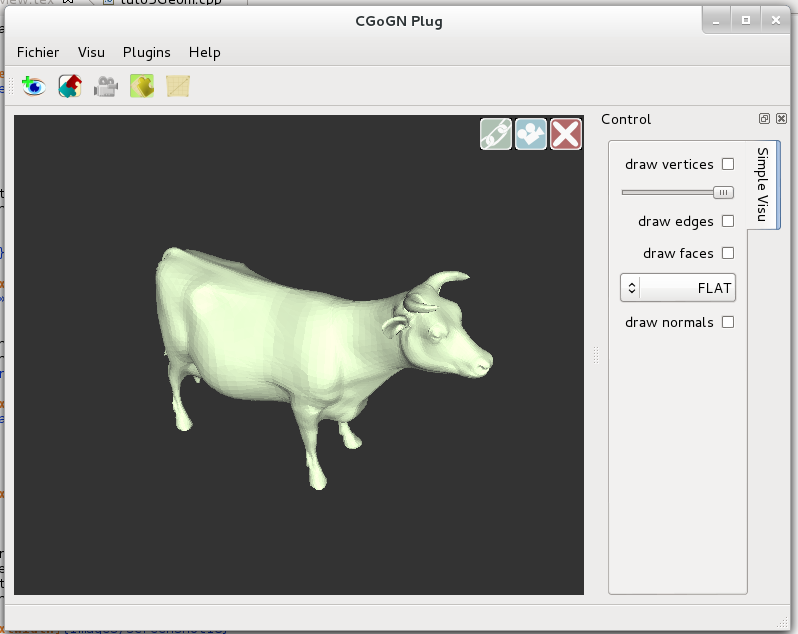
\includegraphics[width=0.7\textwidth]{images/screenshot18}
		\caption{Moo moo mooo.}
	\end{figure}
	\FloatBarrier
	
\subsection{The camera path plugin}
	\paragraph{}
	Another requirement for this project was to be able, given the multiple camera
	gesture, to interpolate a path for a camera from it's successive position
	defined by the user as ``keyframes'', so that the camera could move along this
	path and ``replay'' this movement on the user's demand. Additionally this path
	could be visible for other cameras.
	\begin{figure}[h!p]
		We start with this double visualization of a same scene.\\
		\centering
		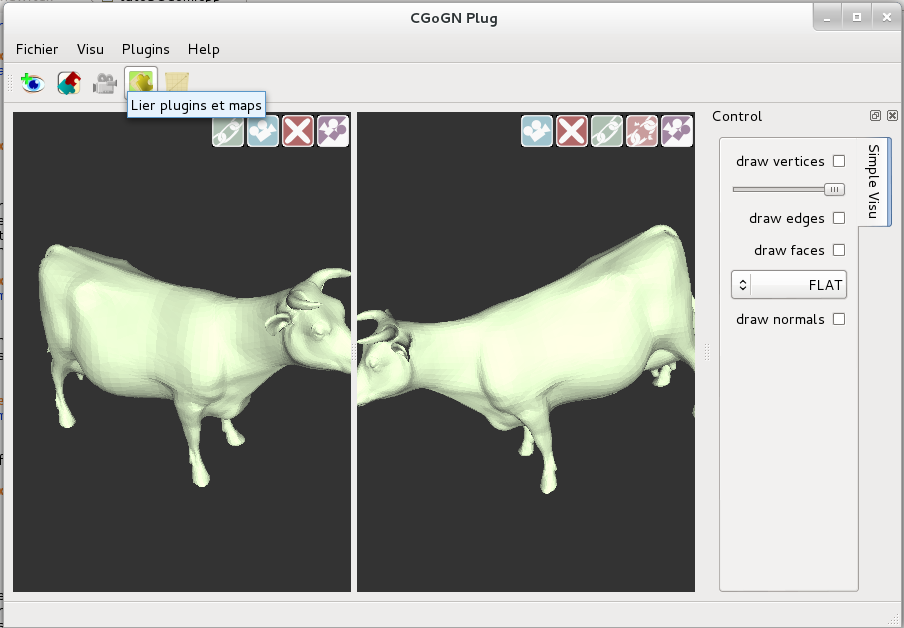
\includegraphics[width=0.9\textwidth]{images/screenshot19}
		\caption{Two moos are better than none.}
	\end{figure}
	\begin{figure}[h!p]
		We now load the ``\textit{cameraPath}'' plugin.\\
		\centering
		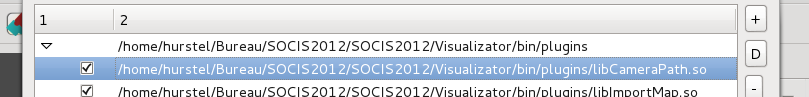
\includegraphics[width=1.0\textwidth]{images/screenshot20}
		\caption{Regular plugin load.}		
	\end{figure}
	\begin{figure}[h!p]
		Linking the existing scene with the plugin.\\
		\centering
		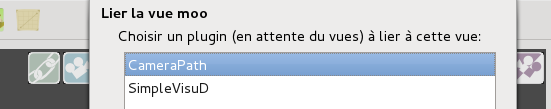
\includegraphics[width=0.7\textwidth]{images/screenshot21}
		\caption{Linking the existing view with the ``\textit{cameraPath}'' plugin.}		
	\end{figure}
	\begin{figure}[h!p]
		A new icon appears on both views.\\
		\centering
		
\includegraphics[width=0.3\textwidth]{images/screenshot22}
		\caption{A wild new icon appears!}		
	\end{figure}
	\begin{figure}[h!p]
		This opens a new dialog where a path can be created using successive
		positions of the camera. Each time the user hits the ``create keyFrame"
		button, a new keyframe, which is the current position of the view's current
		camera, is added to the path. The path is interpolated from this keyframe
		list.\\
		\centering
		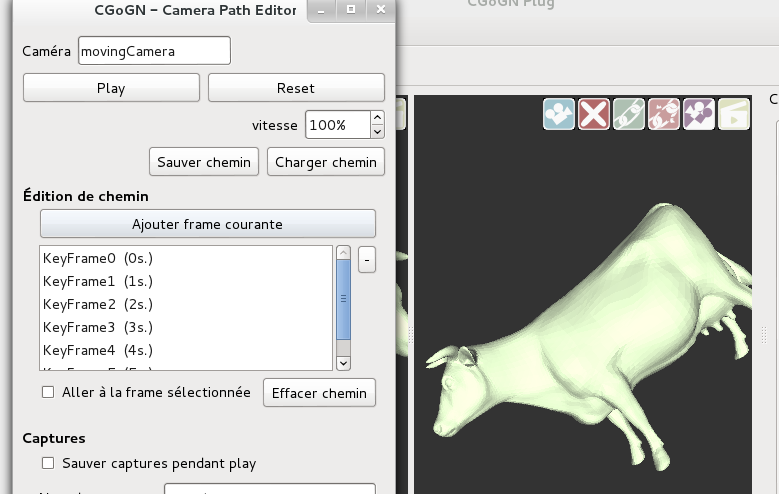
\includegraphics[width=0.9\textwidth]{images/screenshot23}
		\caption{The camera path editor dialog.}		
	\end{figure}
	\begin{figure}[h!p]
		The camera and its interpolated path can both be made visible by other
		cameras from the same scene.\\
		\centering
		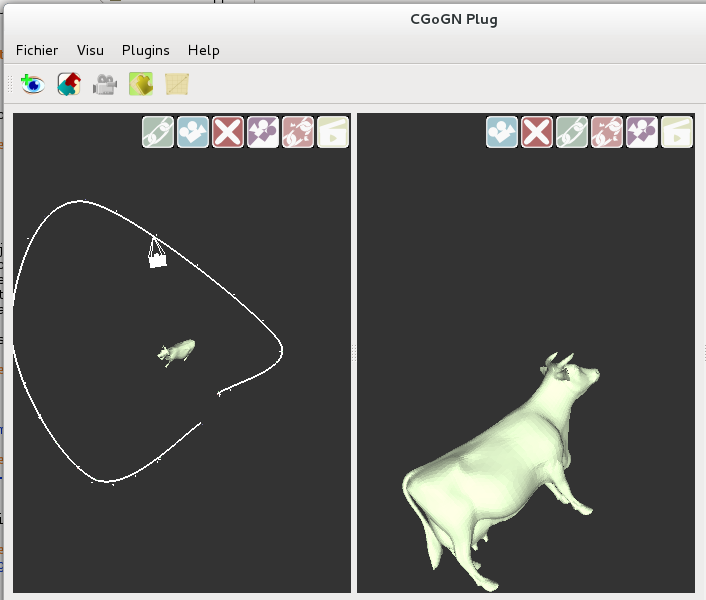
\includegraphics[width=1\textwidth]{images/screenshot24}
		\caption{The path of the second camera viewed by the first.}		
	\end{figure}
	
	\FloatBarrier
	
	\paragraph{}
	A demo video showing how this plugin works may have been joined with this
	document, or may be found in the project's documentation.
	
	
\chapter{How to write plugins?}
\section{Basics and concepts}
	\paragraph{}
	This sections intends to explain the basis to write a visualization plugin. It
	assumes you have knowledge about compilation of C++ \textbf{Qt} files, and also
	uses \href{http://www.cmake.org/}{\textbf{CMake}}, a powerful Makefile
	generating tool. The goal of this section is to write a plugin version of this
	simple \textbf{CGoGN} example:
	\url{http://cgogn.u-strasbg.fr/Wiki/index.php/Tuto_1}
	
\subsection{Visualization concepts}
	\paragraph{}
	Before writing visual plugins there are some main application inner mechanisms
	that need to be understood, that is to say, the way the main application
	manages the different objects of interest and their relations between each
	other: \textbf{Camera}, \textbf{View}, \textbf{Scene} and \textbf{Plugin}.
	\paragraph{Plugin:}
	A plugin is a piece of code written independently to the main application,
	that are loaded and referenced from the main application, and that are
	instantiated as a new object: \textbf{Plugin}. If a plugin has an active
	drawing method, it can draw any visualization but it needs to be linked to
	another object that exists within the main application: a \textbf{Scene}. Note
	that a plugin does not need to be linked to a scene, if it doesn't provide any
	drawing.
	\paragraph{Scene:}
	It's an object that is created by the main application, generally on user's
	demand. A scene isn't actually a drawing object, its aim is to make the link
	between two types of objects: the \textbf{View} and the \textbf{Plugin}. A
	scene can be defined as a set of plugins. A scene exists only for the
	visualization of the plugin drawing methods, so it has to contain at least one
	\textbf{View}. A scene can be linked to several plugins, and a plugin can be
	linked to several scenes.
	\paragraph{View:}
	It's the visualization object that renders the drawings of the plugin that are
	associated to it's parent's \textbf{Scene}. Whereas a scene can have several
	views, a view only have one parent scene. The views can switch between several
	point of views, using \textbf{Camera} objects. A view has at least one camera.
	\paragraph{Camera:}
	This objects can be seen as a point of view. A \textbf{View} has a least one
	camera, and has necessarily an unique ``current'' camera, that is it's current
	point of view. A \textbf{View} can switch between several camera, and it also
	can be considered as a collection of cameras. A \textbf{Camera} can belong to
	several views (from different scenes) at the same time, it is then a ``shared''
	camera.
	\FloatBarrier
	\paragraph{}
	Here is a simple representation of a simple situation: a drawing
	\textbf{Plugin} that is linked to a \textbf{Scene} that is made of an unique
	\textbf{View} containing only one \textbf{Camera} (ie:
	\ref{fig:tuto5GeomView}):
	\begin{figure}[h!p]
		\centering
		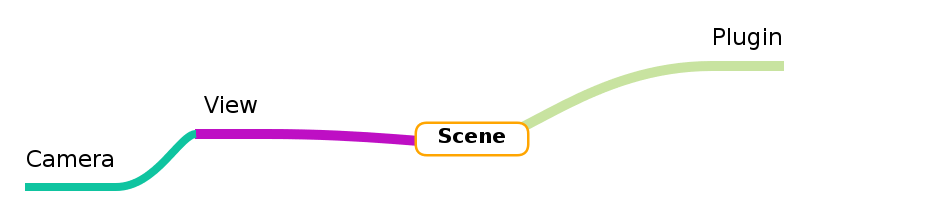
\includegraphics[width=1\textwidth]{images/systemMap1}
		\caption{1 plugin drawing in 1 scene made of 1 view that has 1 camera.}		
	\end{figure}
	\paragraph{}
	Furthermore, a representation of (~\ref{fig:tuto5GeomDoubleView}) would be:
	\begin{figure}[h!p]
		\centering
		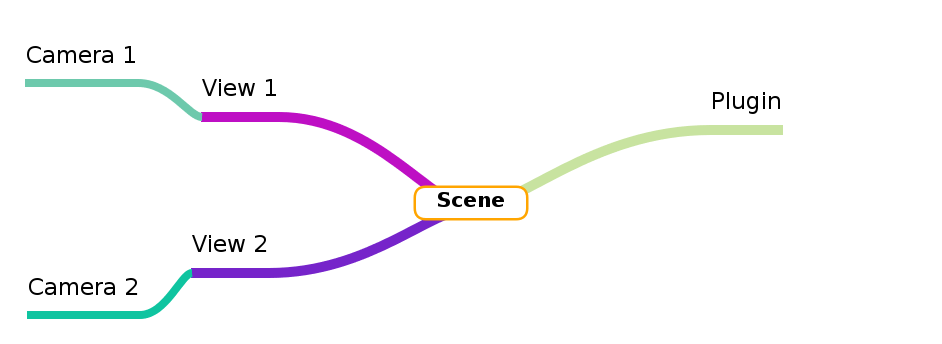
\includegraphics[width=1\textwidth]{images/systemMap2}
		\caption{1 plugin drawing in 1 scene made of 2 views each one working with
		their own camera.}
	\end{figure}
	\FloatBarrier

\subsection{The first plugin}
	\subsubsection{How to write the plugin}
	\paragraph{}
	A good way to comprehend the plugin mechanism is to check the
	\href{http://qt-project.org/doc/qt-4.8/plugins-howto.html}{\textbf{Qt} plugin
	mechanism}, which our plugin system relies on.
	\paragraph{}
	Our plugin is based on a \textbf{CGoGN} tutorial:
	\url{http://cgogn.u-strasbg.fr/Wiki/index.php/Tuto_1}. Here, we will create a
	single visualization plugin that creates in a map a triangle, a square,
	connect them, affect positions to vertices and visualize it. The plugin
	will be called ``\textit{FirstPlugin}", and will be compiled  as a
	dynamic C++ library, that will consequently result in a file called
	``\textbf{libFirstPlugin.so}''. Here's the skeleton for such a plugin:
	\paragraph{firstPlugin.h}~
	\begin{lstlisting}
		#ifndef FIRSTPLUGIN_H_
		#define FIRSTPLUGIN_H_
		
		
		
		#include "visualPlugin.h"
		
		
		/**---CGoGN includes **/
			#include "Utils/Qt/qtSimple.h"
			#include "Utils/cgognStream.h"
		
			#include "Topology/generic/parameters.h"
		
			#ifdef USE_GMAP
				#include "Topology/gmap/embeddedGMap2.h"
			#else
				#include "Topology/map/embeddedMap2.h"
			#endif
		
			#include "Algo/Render/GL2/topoRender.h"
		/**---CGoGN includes **/
		
		
		/**---Definitions  specific to CGoGN ---*/
			using namespace CGoGN ;
		
			/**
			 * Struct that contains some information about the types of the manipulated objects
			 * Mainly here to be used by the algorithms that are parameterized by it
			 */
			struct PFP: public PFP_STANDARD
			{
				// definition of the type of the map
			#ifdef USE_GMAP
				typedef EmbeddedGMap2 MAP;
			#else
				typedef EmbeddedMap2 MAP;
			#endif
			};
		
			typedef PFP::MAP MAP;
			typedef PFP::VEC3 VEC3;
		/**---Definitions  specific to CGoGN ---*/
		
		/**
		 * This class is a basic minimal plugin.
		 * All the methods in this class are overloaded methods.
		 * In order to create a valid plugin, all the method in this
		 * needs to be declared (they are actually overloaded methods
		 * from VisualPlugin), even if your plugin doesn't make any
		 * drawing.
		 */
		
		/**
		 * Our plugin must inherit from VisualPlugin,
		 * that is a class that itself is an implementation
		 * of the Plugin interface (virtual class). It contains
		 * many useful and essential methods.
		 */
		class FirstPlugin : public VisualPlugin{
			/**
			 * Essential Qt macros.
			 */
			Q_OBJECT
			Q_INTERFACES(Plugin)
		public:
			FirstPlugin(){}
			~FirstPlugin(){}
		
			/**
			 * The classical call back for the initGL method
			 * When a scene will be link to this plugin, it will call
			 * back this method with itself as a parameter.
			 */
			void cb_initGL(Scene* scene);
		
			/**
			 * The drawing method that needs to be overloaded.
			 * Each time a scene (that is to say, at least one of the
			 * views that is contains) needs to be refresh, it calls back
			 * this method with itself as a parameter
			 */
			void cb_redraw(Scene* scene);
		
			/**
			 * The plugin's activation method
			 * Each time the main application loads this plugin,
			 * it call this method. Writing this method is
			 * the occasion to initialize the plugin and check certain
			 * conditions.
			 * If this methods return 'false', the plugin load will be aborted.
			 */
			bool activate();
			/**
			 * The plugin's disabling method
			 * Each time the main application will unload the plugin
			 * it will call this method.
			 */
			void disable();
		
		
		protected:
			/** Attributes that are specific to this plugin **/
				MAP myMap;
		
				// attribute for vertices positions
				VertexAttribute<VEC3> position;
		
				// render (for the topo)
				Algo::Render::GL2::TopoRender* m_render_topo;
		
				// just for more compact writing
				inline Dart PHI1(Dart d) { return myMap.phi1(d); }
				inline Dart PHI_1(Dart d) { return myMap.phi_1(d); }
				inline Dart PHI2(Dart d) { return myMap.phi2(d); }
				template<int X>
				Dart PHI(Dart d) { return myMap.phi<X>(d); }
			/** Attributes that are specific to this plugin **/
		};
		
		#endif /* FIRSTPLUGIN_H_ */
	\end{lstlisting}
	\paragraph{}
	And here is the \textit{.cpp} file, that implements these methods:
	\paragraph{firstPlugin.cpp}~
	\begin{lstlisting}
		#include "firstPlugin.h"

		#include "Algo/Geometry/boundingbox.h"
		
		
		bool FirstPlugin::activate(){
			// creation of 2 new faces: 1 triangle and 1 square
				Dart d1 = myMap.newFace(3);
				Dart d2 = myMap.newFace(4);
		
				// sew these faces along one of their edge
				myMap.sewFaces(d1, d2);
		
				// creation of a new attribute on vertices of type 3D vector for position.
				// a handler to this attribute is returned
				position = myMap.addAttribute<VEC3, VERTEX>("position");
		
				// affect position by moving in the map
				position[d1] = VEC3(0, 0, 0);
				position[PHI1(d1)] = VEC3(2, 0, 0);
				position[PHI_1(d1)] = VEC3(1, 2, 0);
				position[PHI<11>(d2)] = VEC3(0, -2, 0);
				position[PHI_1(d2)] = VEC3(2, -2, 0);
		
				m_render_topo=NULL;
		
				return true;
		}
		
		void FirstPlugin::disable(){
			if(m_render_topo){
				delete m_render_topo;
			}
		}
		
		void FirstPlugin::cb_redraw(Scene* scene){
			m_render_topo->drawTopo();
		}
		
		void FirstPlugin::cb_initGL(Scene* scene){
			if(scene){
				//we fit the first (possibly the only) view
				//of the newly linked scene to the content
				//of our map
		
				//  bounding box of scene
				Geom::BoundingBox<PFP::VEC3> bb = Algo::Geometry::computeBoundingBox<PFP>(myMap, position);
		
				scene->firstViewFitSphere(bb.center()[0], bb.center()[1], bb.center()[2], bb.maxSize());
		
		
		
				m_render_topo = new Algo::Render::GL2::TopoRender() ;
		
				// render the topo of the map without boundary darts
				SelectorDartNoBoundary<PFP::MAP> nb(myMap);
				m_render_topo->updateData<PFP>(myMap, position, 0.9f, 0.9f, nb);
		
			}
		}
		
		
		/**
		 * If we want to compile this plugin in debug mode,
		 * we also define a DEBUG macro at the compilation
		 */
		#ifndef DEBUG
			//essential Qt function:
			//arguments are
			//	- the complied name of the plugin
			//	- the main class of our plugin (that extends VisualPlugin)
			Q_EXPORT_PLUGIN2(FirstPlugin, FirstPlugin)
		#else
			Q_EXPORT_PLUGIN2(FirstPluginD, FirstPlugin)
		#endif
	\end{lstlisting}
	
	
	\subsubsection{Compilation}
	\paragraph{}	
	To compile a plugin, the files must be compiled into a C++ dynamic library with
	the plugin's main class compiled as a \textbf{Qt} object using the \textbf{Qt}
	tools.
	\paragraph{}
	Assuming that you are already familiar with \textbf{CMake} and compiling
	\textbf{CGoGN} apps, here's a cmake example, compiling the plugin written
	above:
	\paragraph{CMakeLists.txt}~
	\begin{lstlisting}[language=make]
		#assuming that ${QGLVIEWER_PATH} is the directory
		#where QGLViewer was compiled
		SET(QGLVIEWER_INCLUDE_DIR ${QGLVIEWER_PATH}/QGLViewer)

		#the include directories for CGoGN, common libraries
		#and QGLViewer
		INCLUDE_DIRECTORIES(
			${CGoGN_ROOT_DIR}/include
			${COMMON_INCLUDES}
			${CMAKE_CURRENT_SOURCE_DIR}
			${CMAKE_CURRENT_BINARY_DIR}
			${QGLVIEWER_INCLUDE_DIR}
		)
		
		#assuming that ${CGoGN_PLUG_DIR} is the directory
		#of main application project was compiled
		SET(VISUALPLUGIN_CPP_PATH
			${CGoGN_PLUG_DIR}/plugin/visualPlugin.cpp
		)
		SET(VISUALPLUGIN_H_PATH
			${CGoGN_PLUG_DIR}/plugin/visualPlugin.h
		)
		
		SET( FIRSTPLUGIN_SRC
			${VISUALPLUGIN_CPP_PATH}
		    firstPlugin.cpp
		)
		SET( FIRSTPLUGIN_H
			${VISUALPLUGIN_H_PATH}
		    firstPlugin.h
		)
		
		#using Qt tools to generate the "moc" file for the 
		#plugin Q_OBJECT
		QT4_WRAP_CPP(FIRSTPLUGIN_MOC ${FIRSTPLUGIN_H})
	
		#compiling as a dynamic library
		ADD_LIBRARY(FirstPlugin SHARED
			${FIRSTPLUGIN_SRC}
			${FIRSTPLUGIN_MOC}
		)
	
		#linking with the CGoGN and QGLViewers libraries
		TARGET_LINK_LIBRARIES(FirstPlugin
			${CGoGN_LIBS_R}
			${COMMON_LIBS}
			${QGLVIEWER_INCLUDE_LIBRARY}
		)
	\end{lstlisting}
	
	\paragraph{}
	The compilation should generate our plugin file:
	``\textit{libFirstPlugin.so}''.
	
	\subsubsection{Using the plugin}
	\paragraph{}
	Before using our plugin, we must add it to the main application's plugin
	location list. First we have to open the ``plugin interface''.
	\FloatBarrier
	\begin{figure}[h!p]
		On the left the two first button are respectively to add and individual
		plugin's location, and to add a plugin directory location so that all the
		``\textit{lib*.so}'' files in this directory will be listed.\\
		\centering
		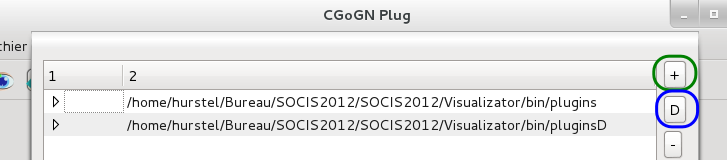
\includegraphics[width=1\textwidth]{images/screenshot25}
		\caption{Add a plugin and add a plugin directory buttons.}
	\end{figure}
	\begin{figure}[h!p]
		We choose the first option, and our load plugin individually.\\
		\centering
		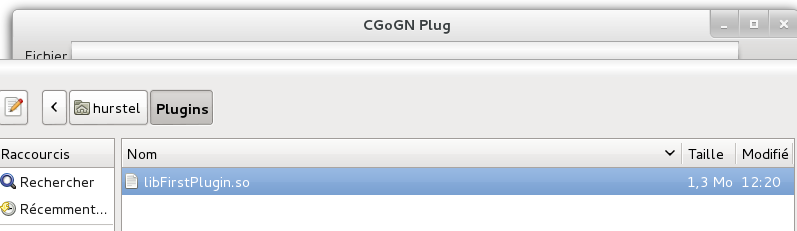
\includegraphics[width=1\textwidth]{images/screenshot26}
		\caption{We select our plugin.}
	\end{figure}
	\begin{figure}[h!p]
		We can now load our plugin and link it to a view.\\
		\centering
		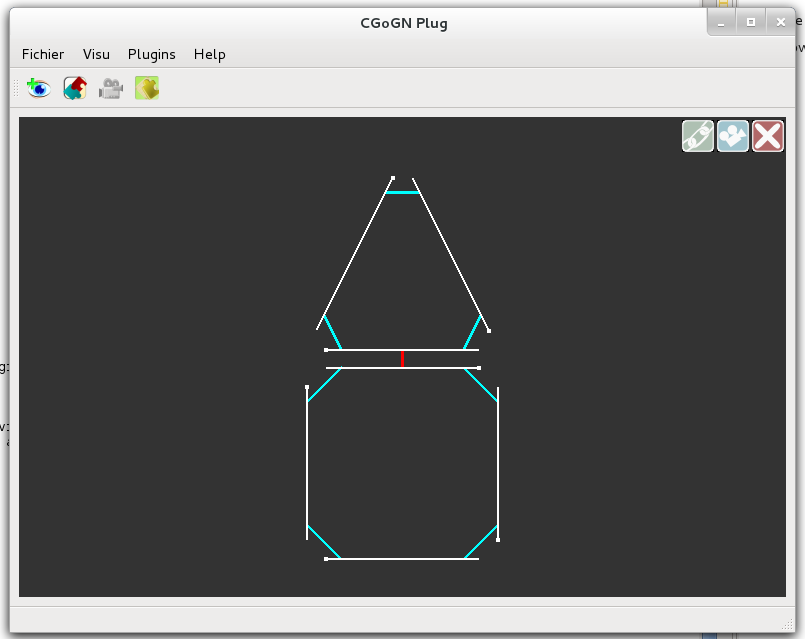
\includegraphics[width=0.7\textwidth]{images/screenshot28}
		\caption{Tadaaaa!}
	\end{figure}
	
	
	
	\FloatBarrier
\subsection{Tricks and advice}
	\subsubsection{Understanding the callBacks}
	To avoid segmentation faults it may be of a good help to understand how the
	plugin's call back methods are called. The figure (~\ref{fig:callBacks}) should
	be of an help.
	\begin{figure}[h!p]
		\centering
		\includegraphics[width=0.9\textwidth]{images/callBacks}
		\caption{The main call backs between the main application and a plugin.}
		\label{fig:callBacks}
	\end{figure}
	
	\subsubsection{Bug \& Debug}
	\paragraph{Common bug:}
	As said before, the compiled are ``\textit{lib*.so}'' files. But sometimes,
	when you try to load one of these files as a plugin, the program may tell you
	that the plugin isn't compatible. Several simple mistakes can be the cause of
	this inconvenience. Here's some advice to avoid it:
	\begin{itemize}
	  \item make sure that all the necessary Qt macros are correctly used:
	  	\begin{itemize}
	   		\item in the plugin's main class declaration:
	  		\texttt{Q\_OBJECT} and \texttt{Q\_INTERFACES(Plugin)}
	  		\item in the plugin's implementation file:
	  		\texttt{Q\_EXPORT\_PLUGIN2(ProgName, MainClassName)}
		\end{itemize}
		\item make sure that you have overloaded each of the four obligatory
		\textbf{VisualPlugin} pure virtual methods:
		\begin{itemize}
		  	\item \texttt{bool activate()}
		  	\item \texttt{void cb\_initGL()}
		  	\item \texttt{void cb\_redraw()}
		  	\item \texttt{void disable()}
		\end{itemize}
		\item make sure that the files containing the declaration and implementation
		of the plugin's main class are compiled as \textbf{Qt} object files.
		\item make sure that each method you declare or overload is
		implemented.
		\item {\em{do not}} redefine (change signature) any of the
		\textbf{VisualPlugin}'s inherited method.
	\end{itemize}
	
	\paragraph{Debug:}
	Naturally a coder will want to test and debug its plugin. If you want to use
	\href{http://www.gnu.org/software/gdb/}{\textbf{GDB}} on your own plugin their
	are a few steps you need to follow:
	\begin{itemize}
	  \item Compile your plugin in debug mode. Be sure that you use the
	  \textbf{debug} version of the CGoGN library. If you have a normal built
	  plugin and a debug built plugin with different names, in your plugin code, be
	  sure to use:
	  \begin{lstlisting}[language=make]
			#ifndef DEBUG
				Q_EXPORT_PLUGIN2(FirstPlugin, FirstPlugin)
			#else
				Q_EXPORT_PLUGIN2(FirstPluginD, FirstPlugin)
			#endif
	  \end{lstlisting}
	  and to define the \texttt{DEBUG} macro in your debug compilation.
	  \item Use a debug compiled version of the main application with \textbf{GDB}
	  \item In \textbf{GDB} before using the \texttt{run} command don't forget to
	  use:
	  \begin{lstlisting}[language=bash]
	  		directory [path_to/the_directory/containing/the_plugin]
	  \end{lstlisting}	  
	\end{itemize}
	If you follow these steps you should be able to debug your plugin using
	\textbf{GDB}.
	
	
\section{Going further\ldots}
	\paragraph{}
	This section aims to present and explain more plugin features and methods in
	order to write more advanced plugins.
	
	\FloatBarrier
\subsection{Few words on plugins}
	\paragraph{}
	As seen in the previous plugin example, a plugin must be an inheritance of a
	virtual class, \textbf{VisualPlugin}, that is itself an inheritance of a
	pure virtual class, considered as a plugin interface (~\ref{fig:plugins}).
	\begin{figure}[h!p]
		\centering
		
\includegraphics[width=0.3\textwidth]{images/plugins}
		\caption{The plugins inheritence graph.}
		\label{fig:plugins}
	\end{figure}
	\paragraph{}
	The point of inheriting an halfway class is that \textbf{VisualPlugin} already
	declares some empty virtual call-back methods so that the plugin coder doesn't
	have to declare the ones he doesn't want to use, but it also provides several
	\textit{ready-to-use} methods that offer many easy to use features, for
	example, add GUI interface, adjust some plugins properties. Many of these methods are
	presented and explained further. 
\subsection{Objects and visualization plugins}
	As you know, one of the main goals of this project is to provide a main
	application that is a mere kernel that needs to be completed with third party
	plugins. The main application provides several objects for visualization and
	interface creation. As told earlier, this application and the plugin systems
	uses \href{http://qt-project.org/}{\textbf{Qt}} and another library
	(also Qt based) \textbf{\href{http://www.libqglviewer.com/}{libQGLviewer}}.
	Here are some precision about the objects of interest that you may have to
	consider for plugin writing.
	
	\subsubsection{Scene:}
	\paragraph{}
	A scene is a drawing that can be made by one or several plugin at the same
	time. A scene can be scene from several point of views (View objects) at the
	same time. That is why a scene is both a collection of plugins and a collection
	of views.
	\paragraph{Automatic creation: }
	As seen earlier, a scene is meant to be created empty (with one view, and
	linked to no plugin) by user, then be linked by the user to an active drawing
	plugin. Although a plugin can automatically create a scene if he calls the
	method:
	\begin{center}
		\texttt{bool addNewScene(QString name, Scene* \&scene)}\\
		or\\
		\texttt{bool addNewSceneDialog(QString name, Scene* \&scene)}
	\end{center}
	The only difference between two methods is that the first automatically places
	the first view of the scene, and the second one opens a dialog to ask the user
	where to place it on the ``view area'' of the application. The effects and
	signatures for these methods use are the same:\\
	\begin{center}
	\begin{tabular}{|l|c|c|p{0.4\textwidth}|}
		\hline
		~ & name & type & description
		\\ \hline
		\textbf{argument:} & name & QString & 
			The name under witch the scene will be referenced in the main application.
		\\ \cline{2-4}
		~ & scene & Scene* \& &
			Once the scene is created, this pointer will be affected with it's memory
			address: it's an out parameter.
		\\ \hline
		\textbf{return:} & ~ & bool &
			A boolean whether the creation of the scene has succeeded or not.
		\\ \hline
	\end{tabular}
	\end{center}
	\textbf{Notes:} 
	\begin{itemize}
	  \item A call to the plugin's \texttt{cb\_intGL()} call back method will be
	  made but not to \texttt{cb\_recieveScene()}.
	  \item When the plugin will be unload, this scene will be destroyed.
	  \item Creating a scene automatically \em{is not recommended}.
	\end{itemize}
	\paragraph{Call-back on scene linking:} We've mentioned several time the
	call-back method:
	\begin{center}
		\texttt{void cb\_recievedScene(Scene* scene)}
	\end{center}
	As you may have guessed, it's a call-back method that is called each time a
	scene is linked to the plugin by the user.\\
	\begin{center}
	\begin{tabular}{|l|c|c|p{0.4\textwidth}|}
		\hline
		~ & name & type & description
		\\ \hline
		\textbf{argument:} & scene & Scene* &
			A pointer on the scene that was linked by the user to the plugin.
		\\ \hline
	\end{tabular}
	\end{center}
	The plugin maintains a list attribute \texttt{l\_recievedScene} that contains
	all the references to the received scene. The \texttt{cb\_recievedScene} method
	is called {\em after} the scene has been added to this list. You do not have
	to, and should not, operate on this list (the only operations that could be
	allowed are sorting or re-ordering the list). Overload this method each time
	you want a specific action to be done, when a scene is linked to your plugin.
	
	\paragraph{}
	Of course their's also a call-back method that is called when the scene is
	unlinked and that works in a similar way:
	\begin{center}
		\texttt{void cb\_removingScene(Scene* scene)}
	\end{center}
	However, be sure to note that this method is called {\em before} the 
	scene is removed from the \texttt{l\_recievedScene} list. Once again 
	you do not have	to, and should not, operate on this list. Overload this method
	each time you want a specific action to be done, when a scene is unlinked from
	your plugin.
	
	\subsubsection{View:}
	\paragraph{}
	The \textbf{View} object is the object that renders the drawing (drawn by one
	or more plugins) that characterize a scene. A view can be considered as a point
	of view, and so a scene can have multiple view, although a view belongs to a
	one and only scene. The view inherits the
	\href{http://www.libqglviewer.com/refManual/classQGLViewer.html}
	{\textbf{QGLViewer}} class (from the
	\textbf{\href{http://www.libqglviewer.com/}{libQGLviewer}} library). So if you
	want to operate directly on a view, be sure to check the library's documentation.
	
	\paragraph{}
	You can access to a scene's views using some of \textbf{Scene}'s public
	methods:
	\begin{center}
		\texttt{int countViews()} \\
	\begin{tabular}{|l|c|c|p{0.4\textwidth}|}
		\hline
		~ & name & type & description
		\\ \hline
		\textbf{return:} & ~ & int &
			The current number of views of a scene.
		\\ \hline
	\end{tabular}
	\\~\\~\\
		\texttt{View* getView(int num)} \\
	\begin{tabular}{|l|c|c|p{0.4\textwidth}|}
		\hline
		~ & name & type & description
		\\ \hline
		\textbf{argument:} & num & int &
			the scene's \textit{num}-th view you want to access.
		\\ \hline
		\textbf{return:} & ~ & View* &
			A pointer to the \textit{num}-th view of the plugin, NULL if the view can't
			be accessed or doesn't exists.
		\\ \hline
	\end{tabular}
	\\~\\~\\
		\texttt{QList<View*> views()}
	\begin{tabular}{|l|c|c|p{0.4\textwidth}|}
		\hline
		~ & name & type & description
		\\ \hline
		\textbf{return:} & ~ & QList$<$View*$>$ &
			A list containing references to all of the scene's views.
		\\ \hline
	\end{tabular}
	\end{center}
	Accessing and operating directly on a scene's view can be critical: be very
	cautious. Although this might be useful in some cases, especially when you
	want to access the current camera's matrices, which is common when you overload
	the callback method \texttt{cb\_updateMatrix(View*)}; if you are already
	familiar with \textbf{CGoGN}'s shaders implementation, the default implementation of the
	method may enlighten you:
	\begin{lstlisting}
		void VisualPlugin::cb_updateMatrix(View* view){
			if(view){
				glm::mat4 model(view->getCurrentModelViewMatrice());
				glm::mat4 proj(view->getCurrentProjectionMatrice());
		
				for(std::set< std::pair<void*, Utils::GLSLShader*> >::iterator it = Utils::GLSLShader::m_registeredShaders.begin();
					it != Utils::GLSLShader::m_registeredShaders.end();
					++it)
				{
					if ((it->first == NULL) || (it->first == this))
					{
						it->second->updateMatrices(proj, model);
					}
				}
			}
		}
	\end{lstlisting}
	
	\subsubsection{Camera:}
	\paragraph{}
	As explained earlier the \textbf{View} object has a collection of
	\textit{Camera} objects. These cameras can be considered as different point of
	views available for a view, of course only one camera is considered current
	for a given view. A camera can be shared by several views, so it's modification
	moreover it's suppression can be critical. Several public methods of the
	\textbf{View} class can be called.
	\begin{center}
		\texttt{Camera* currentCamera()}\\
	\begin{tabular}{|l|c|c|p{0.4\textwidth}|}
		\hline
		~ & name & type & description
		\\ \hline
		\textbf{return:} & ~ & Camera* &
			A pointer to the view's current camera.
		\\ \hline
	\end{tabular}
	\\~\\~\\
		\texttt{QList<Camera*> cameras()}\\
	\begin{tabular}{|l|c|c|p{0.4\textwidth}|}
		\hline
		~ & name & type & description
		\\ \hline
		\textbf{return:} & ~ & QList$<$Camera*$>$ &
			A list containing references to all the cameras of the view.
		\\ \hline
	\end{tabular}
	\\~\\~\\
		\texttt{int countCameras()}\\
	\begin{tabular}{|l|c|c|p{0.4\textwidth}|}
		\hline
		~ & name & type & description
		\\ \hline
		\textbf{return:} & ~ & int &
			The number of cameras for the view.
		\\ \hline
	\end{tabular}
	\end{center}
	The class \textbf{Camera} inherits the class
	\href{http://www.libqglviewer.com/refManual/classqglviewer_1_1Camera.html}
	{\textbf{qglviewer::Camera}} provided by the \textbf{libQGLViewer} library. If
	you want to operate correctly on cameras you might want to check it's
	documentation, but again, it also might be critical.
	
\subsection{GUI and user interactions}
	\subsubsection{Custom widgets and menu entries}
	\paragraph{}
	Of course the plugins also offers the possibility to add you own menu entries,
	buttons in the toolbar and custom widget in the main application's dock.
	Although these features requires the basics of \textbf{Qt}'s custom slots and
	custom widget creation.
	
	\paragraph{Custom menu entries:}
	Their are two usable methods provided by the inheritance to
	\textbf{VisualPlugin} that allows you to add your custom menu entries:
	\begin{center}
		\texttt{QAction* addMenuAction(QString menuPath, const char* method)}
	\begin{tabular}{|l|c|c|p{0.6\textwidth}|}
		\hline
		~ & name & type & description
		\\ \hline
		\textbf{argument:} & menuPath & QString &
			The ``menu path'' for your custom entry matching this pattern:
			\textit{:menu/submenu1/submenu2/myEntry}. For example if your menu path is
			\textit{:file/export/image}, in will create a submenu ``export'', in the
			``file'' menu, that contain the entry image. Any non existing menu or submenu
			is created by this method.
		\\
		\cline{2-4}
		~ & method & const char* &
			The \textbf{Qt} slot you want to connect to your menu entry. For example if
			you want the slot ``\texttt{exportImage()}'' to be called when the custom
			entry is clicked, this argument should be ``SLOT(exportImage())''.
		\\ \hline
		\textbf{return:} & ~ & QAction* &
			A reference to the Qt's ``action'' object that has been created by this
			method. NULL if the method fails.
		\\ \hline
	\end{tabular}
	\end{center}
	This method creates automatically your ``action'' object that is used to
	connect your entry with one of your slots. Although you might want to connect a
	same action to several menu entries or a to a toolbar button. In that case you
	you can declare your own QAction instance, and use this method:
	\begin{center}
		\texttt{bool addMenuAction(QString menuPath, QAction* action)}
	\begin{tabular}{|l|c|c|p{0.6\textwidth}|}
		\hline
		~ & name & type & description
		\\ \hline
		\textbf{argument:} & menuPath & QString &
			The ``menu path'' for your custom entry matching this pattern:
			\textit{:menu/submenu1/submenu2/myEntry}. For exemple if your menu path is
			\textit{:file/export/image}, in will create a submenu ``export'', in the
			``file'' menu, that contain the entry image. Any non existing menu or submenu
			is created by this method.
		\\
		\cline{2-4}
		~ & method & QAction* &
			A pointer on the QAction you want to connect to your custom entry.
		\\ \hline
		\textbf{return:} & ~ & bool &
			True if the method succeeded, false otherwise.
		\\ \hline
	\end{tabular}
	\end{center}
	
	\paragraph{Custom toolbar buttons:}
	In a similar way \textbf{VisualPlugin} provides inherited methods that can be
	used to add custom toolbar buttons:
	\begin{center}
		\texttt{QAction* addToolbarAction(const char* method, QIcon icon= QIcon())}
	\begin{tabular}{|l|c|c|p{0.6\textwidth}|}
		\hline
		~ & name & type & description
		\\ \hline
		\textbf{argument:} & method & const char* &
			The \textbf{Qt} slot you want to connect to your toolbar button. For example
			if you want the slot ``\texttt{exportImage()}'' to be called when the custom
			entry is clicked, this argument should be ``SLOT(exportImage())''
		\\ \cline{2-4}
		~ & icon & QIcon &
			The \textbf{Qt}'s icon of your custom button, an empty icon by default.
		\\ \hline
		\textbf{return:} & ~ & QAction* &
			A reference to the Qt's ``action'' object that has been created by this
			method. NULL if the method fails.
		\\ \hline
	\end{tabular}
	\end{center}
	In the same way than before, there's also a method where you passes an already
	created QAction instance:
	\begin{center}
		\texttt{bool addToolbarAction(QAction* action)}
	\begin{tabular}{|l|c|c|p{0.6\textwidth}|}
		\hline
		~ & name & type & description
		\\ \hline
		\textbf{argument:} & action & QAction* &
			A pointer on the QAction you want to connect to your custom entry.
		\\ \hline
		\textbf{return:} & ~ & bool &
			True if the method succeeded, false otherwise.
		\\ \hline		
	\end{tabular}
	\end{center}
	This last method considers that their's already a QIcon object associated with
	you the QAction object you passed as parameter.
	
	\paragraph{Custom widgets:}
	The following method supposes that you are already familiar with how to create
	(and compile) custom \textbf{Qt} widgets. The main application possesses a dock
	where widgets can be add as new tabs in the dock's area. This method allows
	you to add such widgets:
	\begin{center}
		\texttt{bool addWidgetInDockTab(QWidget* newTabWidget, QString tabText)}
	\begin{tabular}{|l|c|c|p{0.6\textwidth}|}
		\hline
		~ & name & type & description
		\\ \hline
		\textbf{argument:} & newTabWidget & QWidget* &
			A reference to the custom widget you want to add as a new tab in the main
			application's dock.
		\\ \cline{2-4}
		~ & tabText & QString &
			The text that appears on the tab that contains your custom widget.
		\\ \hline
		\textbf{return:} & ~ & bool &
			True if the method succeeded, false otherwise.
		\\ \hline
	\end{tabular}
	\end{center}
	
	\subsubsection{User interactions}
	\paragraph{}
	Of course a plugin coder will want to control the behavior when mouse or
	keyboard actions are detected on a view of a scene. Naturally the
	\textbf{VisualPlugin} class that your plugin must inherit provides
	callback methods that you can overload. It is believe that these methods names
	are explicit enough so that they don't need to be described:
	\begin{itemize}
	  \item \texttt{bool cb\_keyPress(Scene* scene, int event)}
	  \item \texttt{bool cb\_keyRelease(Scene* scene, int event)}
	  \item \texttt{bool cb\_mousePress(Scene* scene, int button, int x, int y)}
	  \item \texttt{bool cb\_mouseRelease(Scene* scene, int button, int x, int y)}
	  \item \texttt{bool cb\_mouseClick(Scene* scene, int button, int x, int y)}
	  \item \texttt{bool cb\_mouseMove(Scene* scene, int buttons, int x, int y)}
	  \item \texttt{bool cb\_wheelEvent(Scene* scene, int delta, int x, int y)}
	\end{itemize}
	You will notice that all of these callback methods must return a boolean. If
	they return false, then the default behavior of a
	\href{http://www.libqglviewer.com/refManual/classQGLViewer.html}
	{\textbf{QGLViewer}} object (\textbf{View} inherits the QGLViewer class) will
	be adopted.
	
\subsection{Maps and VBOs}
	\paragraph{}
	Their is a last feature that has already been shown in a previous example
	(~\ref{fig:linkMapPlugin}) but hasn't been detailed yet: sharing between
	plugins through the main application. This subsection explains how to make the
	\textbf{CGoGN} maps created within a plugin available for other and how to
	attach VBOs to them. Once again, the following assumes that you are already
	familiar with the \textbf{CGoGN} maps and VBO implementation.
	
	\subsubsection{Map and VBO handling types}
	\paragraph{}
	Maps are the main object of interest of the \textbf{CGoGN} library. Plugins are
	supposed to offer functionalities, and specific treatments on the geometric
	object provided by CGoGN. This is why it is necessary that several plugins can
	work on a same map.
	
	\paragraph{}
	VBOs are essential datas if you want to render maps and thus their number is
	limited within \textbf{OpenGL} application. This is why it is interesting to
	allow maps to carry their VBOs so they can also provide them to other plugins
	and not to let each plugin create and allocate their own VBO objects for
	rendering one and only map.
	
	\paragraph{MapHandler:}
	It's the type that handles CGoGN's map. It basicaly is a class that associate a
	reference to a generic map type (\textbf{CGoGN::GenericMap}) with a list of VBO
	references. Here are the constructor and the main useful methods of the
	\textbf{MapHandler} class:
	\begin{center}
		\texttt{MapHandler(CGoGN::GenericMap* map)}
	\begin{tabular}{|l|c|c|p{0.5\textwidth}|}
		\hline
		~ & name & type & description
		\\ \hline
		\textbf{argument:} & map & CGoGN::GenericMap* &
			A reference to an allocated CGoGN generic map
		\\ \hline
	\end{tabular}
	\\~\\~\\
		\texttt{CGoGN::GenericMap* map()}
	\begin{tabular}{|l|c|c|p{0.5\textwidth}|}
		\hline
		~ & name & type & description
		\\ \hline
		\textbf{return:} & ~ & CGoGN::GenericMap* &
			A reference to the CGoGN map contained by the current MapHandler.
		\\ \hline
	\end{tabular}
	\end{center}
	The VBO also possess their own handling type \textbf{VBOHandler} that will be
	detailed further. Here are how to access these object from a
	\textbf{MapHandler} instance.
	\begin{center}
		\texttt{VBOHandler* findVBO(QString name)}
	\begin{tabular}{|l|c|c|p{0.6\textwidth}|}
		\hline
		~ & name & type & description
		\\ \hline
		\textbf{argument:} & name & QString &
			The name of the VBO you want to access.
		\\ \hline
		\textbf{return:} & ~ & VBOHandler* &
			A reference to the VBO associate to the given name, NULL if such a VBO isn't
			associated with the generic map handled by this object.
		\\ \hline
	\end{tabular}
	\\~\\~\\
		\texttt{QList<VBOHandler*> findVBOsMatching(QRegExp regexp)}
	\begin{tabular}{|l|c|c|p{0.6\textwidth}|}
		\hline
		~ & name & type & description
		\\ \hline
		\textbf{argument:} & regexp & QRegExp &
			A regular expression to match the names of the VBOs you want to access.
		\\ \hline
		\textbf{return:} & ~ & VBOHandler* &
			A reference to the VBO associate matching the regular expression.
		\\ \hline
	\end{tabular}
	\\~\\~\\
		\texttt{bool addVBO(VBOHandler* vboH)}
	\begin{tabular}{|l|c|c|p{0.4\textwidth}|}
		\hline
		~ & name & type & description
		\\ \hline
		\textbf{argument:} &  vboH & VBOHandler* &
			A reference to an handled vbo you want want to associate with the map handled
			by this object.
		\\ \hline
		\textbf{return:} &  ~ & bool &
			A boolean whether or not the method has succeeded.
		\\ \hline
	\end{tabular}
	\\~\\~\\
		\texttt{VBOHandler* addNewVBO(QString vboName)}
	\begin{tabular}{|l|c|c|p{0.5\textwidth}|}
		\hline
		~ & name & type & description
		\\ \hline
		\textbf{argument:} & vboName & QString &
			A name for the VBO you want to create and associate with the map handled by
			this object. Typically the name matches this pattern:
			``\textit{[function]VBO}''. For example, for a position VBO the name should
			be ``\textit{positionVBO}'', for a normal VBO ``\textit{normalVBO}''.
		\\ \hline
		\textbf{return:} &  ~ & bool &
			A reference to the handler of the newly created VBO, NULL if the method
			fails, typically if a VBO with a same name as the given name already exists.
		\\ \hline
	\end{tabular}
	\\~\\~\\
		\texttt{VBOHandler* takeVBO(VBOHandler* vbo)}
	\begin{tabular}{|l|c|c|p{0.5\textwidth}|}
		\hline
		~ & name & type & description
		\\ \hline
		\textbf{argument:} & vbo & VBOHandler* &
			A pointer to the handler VBO you want to disassociate to the map handled by
			the current object.
		\\ \hline
		\textbf{return:} &  ~ & bool &
			A reference to the handler no longer associate to the map handled by
			the current object, NULL if failure.
		\\ \hline
	\end{tabular}
	\\~\\~\\
		\texttt{int countVBO()}
	\begin{tabular}{|l|c|c|p{0.5\textwidth}|}
		\hline
		~ & name & type & description
		\\ \hline
		\textbf{return:} & ~ & int &
			The number of VBOs associated to the map handled by
			the current object.
		\\ \hline
	\end{tabular}	
	\end{center}
	
	\paragraph{VBOHandler:}
	Basically it's the type that handles VBO by associating them to a recognizable
	name. Actually this class extends \textbf{CGoGN}'s VBO class
	(\textbf{CGoGN::Utils::VBO}) and contains attributes such as his name and a
	list of reference to instances of \textbf{MapRender} class the VBO is
	associated with. Here are \textbf{VBOHandler}'s useful constructors and public
	methods you'll have to use if you want to render shared maps using VBOs:
	\begin{center}
		\texttt{VBOHandler(QString name)}
	\begin{tabular}{|l|c|c|p{0.5\textwidth}|}
		\hline
		~ & name & type & description
		\\ \hline
		\textbf{argument:} & name & QString &
			The name associated to the newly created VBO this object will handle.
		\\ \hline
	\end{tabular}
	\\~\\~\\
		\texttt{VBOHandler(VBO vbo, QString name)}
	\begin{tabular}{|l|c|c|p{0.5\textwidth}|}
		\hline
		~ & name & type & description
		\\ \hline
		\textbf{argument:} & vbo & VBO &
			A CGoGN vbo that will be handled by this object
		\\ \cline{2-4}
		~ & name & QString &
			The name associated to the VBO this object will handle.
		\\ \hline
	\end{tabular}
	\\~\\~\\
		\texttt{bool isShared()}
	\begin{tabular}{|l|c|c|p{0.5\textwidth}|}
		\hline
		~ & name & type & description
		\\ \hline
		\textbf{return:} & ~ & bool &
			A boolean whether or not this handled VBO is shared between two or more
			instance of \textbf{MapHandler}.
		\\ \hline
	\end{tabular}
	\\~\\~\\
		\texttt{QString getName()}
	\begin{tabular}{|l|c|c|p{0.5\textwidth}|}
		\hline
		~ & name & type & description
		\\ \hline
		\textbf{return:} & ~ & QString &
			The name which is associated to the handled VBO.
		\\ \hline
	\end{tabular}
	\end{center}
	\textbf{Important note:} Be sure to remember that VBO object \textbf{must} be
	created withing an \textbf{OpenGL} context, that is to say either within the
	\texttt{cb\_initGL(Scene*)} method either within \texttt{cb\_redraw(Scene*)}.
	
	\subsubsection{Sharing maps}
	\paragraph{}
	The idea is that any plugin can create a map and then
	reference it into the main application that can then share it with other
	plugins on user's demand. The procedure within a plugin is:
	\begin{enumerate}
	  \item create a \textbf{CGoGN} map
	  \item handle the map with a \textbf{MapHandler} class instance.
	  \item create and handle VBO using the \textbf{VBO} handler class.
	  \item associate the handled VBOs to the map
	  \item send the \textbf{MapHandler} object to the main application so that it
	  will reference it and make it available for other plugins.
	\end{enumerate}
	\paragraph{}
	Here are the methods provided by
	\textbf{VisualPlugin} that you'll have to call in order to send a
	\textbf{MapHandler} object to the main application:
	\begin{center}
		\texttt{bool addReferencedMap(QString map\_name, MapHandler* map)}
	\begin{tabular}{|l|c|c|p{0.5\textwidth}|}
		\hline
		~ & name & type & description
		\\ \hline
		\textbf{argument:} & map\_name & QString &
			The name under which the main application will reference the
			handled map.
		\\ \cline{2-4}
		~ & map & MapHandler* & 
			The reference to handler of the map you want to made available for sharing.
		\\ \hline
		\textbf{return:} & ~ & bool &
			A boolean whether or not the method succeeds. For example, failure if
			another map is already referenced under the same name.
		\\ \hline
	\end{tabular}
	\\~\\~\\
		\texttt{MapHandler*  getReferencedMap(QString map\_name)}
	\begin{tabular}{|l|c|c|p{0.5\textwidth}|}
		\hline
		~ & name & type & description
		\\ \hline
		\textbf{argument:} & map\_name & QString &
			The name of the map handler referenced by the main application.
		\\ \hline
		\textbf{return:} & ~ & MapHandler* & 
			A pointer to the map handler referenced by the main application under the
			given name, NULL is failure, for example if no map handler is referenced
			under this name
		\\ \hline
	\end{tabular}	
	\end{center}
	\textbf{Note: } Since the map are meant to be shared manually between plugins
	by the user, the last method shouldn't be useful.
	
	\subsubsection{Plugins maps callback}
	\paragraph{}
	In a similar way than callbacks methods are called when a user links a scene to
	a plugin, callbacks methods are called when maps are shared with plugins.A
	coder will probably want to runs specific code when the user share a map with
	his plugin. To do so, \textbf{VisualPlugin} provides the following callback
	methods that the code only have to overload:
	\begin{itemize}
	  \item \texttt{void cb\_recievedMap(MapHandler* map)}
	  \item \texttt{void cb\_removingMap(MapHandler* map)}
	\end{itemize}
	The two methods are respectively called when the user shares the map handled by
	the map handler given as a parameter with the current plugin.
	\paragraph{}
	The \textbf{VisualPlugin} class maintains a list \texttt{l\_map} containing the
	references to all the map handlers that handle the map shared with the plugin.
	Be sure \textbf{not to} remove any element of this list with you own code. The
	only permitted operation that could be allowed are sorting or re-ordering the
	list.
	\paragraph{}
	Finally it's important that you know that the \texttt{cb\_recievedMap()} is
	called \textbf{after} the map handler is added to \texttt{l\_map} and that
	\texttt{cb\_removingMap()} is called \textbf{before} the map handler is removed
	from this list.
\end{document}